\documentclass[11pt,a4paper]{report}
\usepackage[spanish,es-nodecimaldot]{babel}	% Utilizar español
\usepackage[utf8]{inputenc}					% Caracteres UTF-8
\usepackage{graphicx}						% Imagenes
\usepackage[hidelinks]{hyperref}			% Poner enlaces sin marcarlos en rojo
\usepackage{fancyhdr}						% Modificar encabezados y pies de pagina
\usepackage{float}							% Insertar figuras
\usepackage[textwidth=390pt]{geometry}		% Anchura de la pagina
\usepackage[nottoc]{tocbibind}				% Referencias (no incluir num pagina indice en Indice)
\usepackage{enumitem}						% Permitir enumerate con distintos simbolos
\usepackage[T1]{fontenc}					% Usar textsc en sections
\usepackage{amsmath}						% Símbolos matemáticos
\usepackage{listings}
\usepackage{longtable}
\usepackage{subcaption}
\usepackage{datatool}
\usepackage{filecontents}


% Comando para poner el nombre de la asignatura
\newcommand{\asignatura}{Simulación de Sistemas}
\newcommand{\autor}{Adrián Acosa Sánchez}
\newcommand{\titulo}{PRÁCTICA 3}
\newcommand{\subtitulo}{Modelos de Simulación Dinámicos y Discretos}
\newcommand{\rama}{Computación y Sistemas Inteligentes}

% Configuracion de encabezados y pies de pagina
\pagestyle{fancy}
\lhead{\autor{}}
\rhead{\asignatura{}}
\lfoot{Grado en Ingeniería Informática}
\cfoot{}
\rfoot{\thepage}
\renewcommand{\headrulewidth}{0.4pt}		% Linea cabeza de pagina
\renewcommand{\footrulewidth}{0.4pt}		% Linea pie de pagina

\usepackage{graphicx}
\begin{document}
\pagenumbering{gobble}

% Pagina de titulo
\begin{titlepage}

\begin{minipage}{\textwidth}

\centering

%
\includegraphics[scale=0.5]{img/ugr.png}\\

\includegraphics[scale=0.3]{img/logo_ugr.jpg}\\[1cm]

\textsc{\Large \asignatura{}\\[0.2cm]}
\textsc{GRADO EN INGENIERÍA INFORMÁTICA}\\[1cm]

\noindent\rule[-1ex]{\textwidth}{1pt}\\[1.5ex]
\textsc{{\Huge \titulo\\[0.5ex]}}
\textsc{{\Large \subtitulo\\}}
\noindent\rule[-1ex]{\textwidth}{2pt}\\[3.5ex]

\end{minipage}

%\vspace{0.5cm}
\vspace{0.7cm}

\begin{minipage}{\textwidth}

\centering

\textbf{Autor}\\ {\autor{}}\\[2.5ex]
\textbf{Rama}\\ {\rama}\\[2.5ex]
\vspace{0.3cm}


\includegraphics[scale=0.3]{img/etsiit.jpeg}

\vspace{0.7cm}
\textsc{Escuela Técnica Superior de Ingenierías Informática y de Telecomunicación}\\
\vspace{1cm}
\textsc{Curso 2022-2023}
\end{minipage}
\end{titlepage}

\pagenumbering{arabic}
\tableofcontents
\thispagestyle{empty}				% No usar estilo en la pagina de indice

\newpage

\setlength{\parskip}{1em}

\chapter{Mi Segundo Modelo de Simulación Discreto}
\newpage
\section{Ejecución del modelo}

Antes de empezar, ejecutaré tanto el modelo con incremento fijo como con incremento variable con los mismos datos. Usaré un número fijo de clientes a atender (el que se propone en el guión) y las siguientes medidas de tiempo para las distintas ejecuciones del mismo:

\begin{itemize}
	\item{tlleg = 0.15, tserv = 0.1 (horas)}
	\item{tlleg = 4.5, tserv = 3 (medias horas)}
	\item{tlleg = 6.75, tserv = 4.5 (cuartos de horas)}
	\item{tlleg = 9, tserv = 6 (minutos)}
	\item{tlleg = 540, tserv = 360 (segundos)}
	\item{tlleg = 5400, tserv = 3600 (décimas de segundo)}
	\item{tlleg = 54000, tserv = 3600 (milésimas de segundo)}
\end{itemize}

Cada modelo de tiempo lo ejecutaremos mil veces y haremos una media con los valores obtenidos. Una vez establecidos los datos para las ejecuciones, procedemos a ver los resultados obtenidos para el modelo con incremento fijo del tiempo.

\newpage
\subsection{Incremento fijo del tiempo}

Los datos obtenidos en el caso del incremento fijo del tiempo son los siguientes:

\begin{tabular}{|c|c|c|c|c|}
\hline
	\texttt{tlleg} & \texttt{tserv} & \textbf{\begin{tabular}[c]{@{}c@{}}Media de\\ porcent. ocio\end{tabular}} & \textbf{\begin{tabular}[c]{@{}c@{}}Media de\\ clientes en cola\end{tabular}} & \textbf{\begin{tabular}[c]{@{}c@{}}Media de tiempo\\ de ejecución (seg.)\end{tabular}}\\
\hline
	0.15 & 0.1 & 0.01289676 & 0 & 0.00077048043 \\
\hline
	4.5 & 3 & 31.742317 & 1.260239 & 0.00081458839\\
\hline
	6.75 & 4.5 & 32.814245 & 1.2912124 & 0.00108435556\\
\hline
	9 & 6 & 32.901228 & 1.3155765 & 0.0009692193\\
\hline
	540 & 360 & 33.182336 & 1.3335208 & 0.0067238491\\
\hline
	5400 & 3600 & 33.338336 & 1.3386199 & 0.06656899\\
\hline
	54000 & 36000 & 33.186988 & 1.3291968 & 0.58698766\\
\hline
\end{tabular}

\begin{figure}[H]
	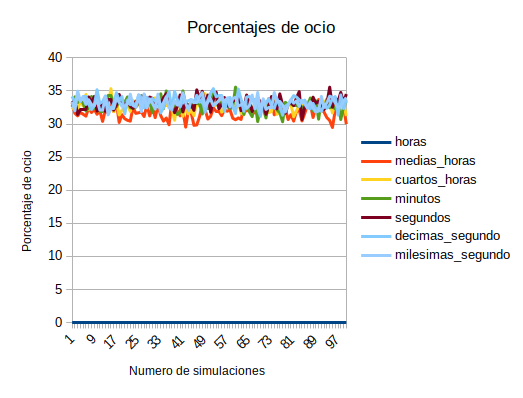
\includegraphics[width=\textwidth]{img/cap-1/porcentaje_de_ocio_fijo.png}
  	\caption{Porcentaje de ocio con incremento del tiempo fijo.}
\end{figure}

\begin{figure}[H]
    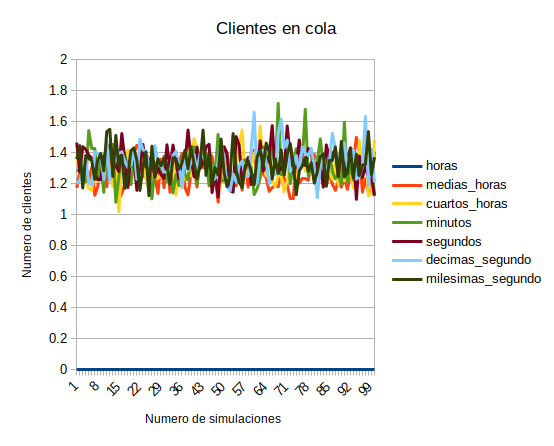
\includegraphics[width=\textwidth]{img/cap-1/tiempo_medio_en_cola_fijo.png}
  	\caption{Numero de clientes en cola con incremento fijo del tiempo.}
\end{figure}

En este caso podemos ver cómo a medida de que disminuimos el tiempo de llegada y de servicio, el porcentaje de ocio crece hasta llegar a un valor medianamente estable al igual que la media de clientes en cola. Sin embargo en el caso de usar horas, no se llegan a quedar clientes esperando. 

\newpage
\subsection{Incremento variable del tiempo}

Los datos obtenidos para el caso del incremento variable del tiempo son los siguientes:

\begin{tabular}{|c|c|c|c|c|}
\hline
	\texttt{tlleg} & \texttt{tserv} & \textbf{\begin{tabular}[c]{@{}c@{}}Media de\\ porcent. ocio\end{tabular}} & \textbf{\begin{tabular}[c]{@{}c@{}}Media de\\ clientes en cola\end{tabular}} & \textbf{\begin{tabular}[c]{@{}c@{}}Media de tiempo\\ de ejecución (seg.)\end{tabular}}\\
\hline
	0.15 & 0.1 & 81.136741 & 6.357511 & 0.00050316099 \\
\hline
	4.5 & 3 & 33.535384 & 1.3574975 & 0.00108329201\\
\hline
	6.75 & 4.5 & 33.599787 & 1.3409273 & 0.00073598041\\
\hline
	9 & 6 & 33.40902 & 1.333977 & 0.00073813895\\
\hline
	540 & 360 & 33.259578 & 1.3370123 & 0.00072627794\\
\hline
	5400 & 3600 & 33.294838 & 1.3506606 & 0.00072098029\\
\hline
	54000 & 36000 & 33.322672 & 1.3340578 & 0.00074971501\\
\hline
\end{tabular}

\begin{figure}[H]
	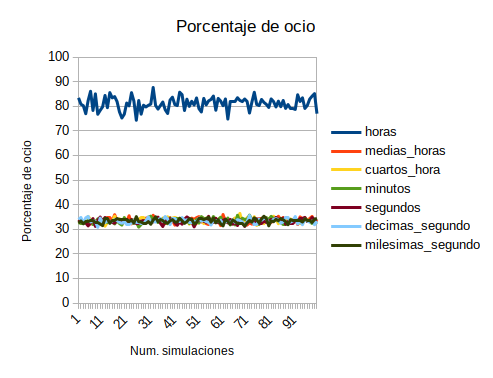
\includegraphics[width=\textwidth]{img/cap-1/porcentaje_de_ocio_variable.png}
  	\caption{Porcentaje de ocio con incremento del tiempo variable.}
\end{figure}

\begin{figure}[H]
    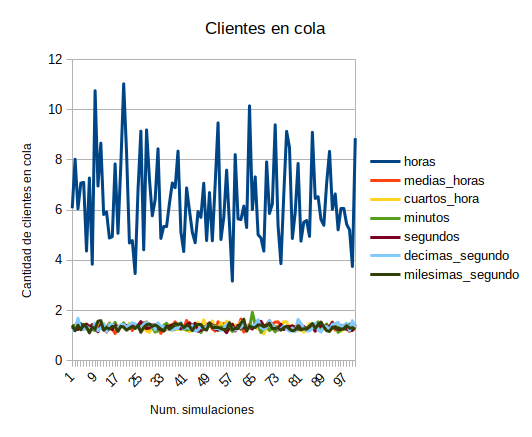
\includegraphics[width=\textwidth]{img/cap-1/tiempo_medio_en_cola_variable.png}
  	\caption{Numero de clientes en cola con incremento variable del tiempo.}
\end{figure}

En este caso, son las horas las que se ven más perjudicadas. Ésto se refleja en que el porcentaje de ocio y el número de clientes en cola es considerablemente más alto que para el resto.

Comparando los resultados obtenidos con los valores teóricos:

\begin{equation}
	\rho = \frac{\texttt{tserv}}{\texttt{tlleg}} = \frac{0.1}{0.15} = 0.66667
\end{equation}

\begin{equation}
	Q(n) \rightarrow \frac{0.66667^2}{1-0.66667} = 1.33335
\end{equation}

\begin{equation}
	PTO(n) = 100*(1-\rho) = 100*(1-0.66667) = 33.33333
\end{equation}


\newpage
Viendo los resultados obtenidos por los cálculos teóricos nos damos cuenta de que a la hora de simular el modelo con un tiempo de simulación de horas los resultados obtenidos no son nada cercanos a lo esperable, y por lo tanto no sería una buena medida de tiempo para simularlo.

En el caso del resto de medidas, vemos que obtenemos valores muy similares al cálculo teórico de $PTO(n)$ y de $Q(n)$ en la simulación con el incremento variable del tiempo. En el caso del incremento fijo hay más variación a medida que tomamos tiempos de llegada y servicio más altos que los segundos. Con tiempos más cortos que los segundos vemos que el sistema se acerca mucho a lo esperado.

Como conclusión, si queremos simular este modelo con tiempos de llegada y de servicio más grandes que los segundos, lo ideal sería usar una simulación con incremento del tiempo variable en lugar de incrementos fijos debido a la similitud con los valores teóricos. Para tiempos de llegada y servicio más cortos, si nos fijamos en el tiempo de ejecución, lo mejor sería usar el método de incremento variable del tiempo también ya que la simulación es bastante más rápida en cualquiera de los casos, aunque si nos da igual este parámetro podríamos elegir cualquier tipo de incremento.

\newpage

\chapter{Mi Tercer Modelo de Simulación}
\newpage

\section{Probando el modelo}

En primer lugar, en el guión se pide buscar un valor de número de simulaciones donde los resultados sean relativamente estables. Para ello lo que he hecho ha sido simular dicho modelo obteniendo uno de los valores que proporciona el informe del modelo y compararlo al ejecutarlo diferentes números de veces para ver a partir de qué valor de número de simulaciones puedo considerarlo relativamente estable. La siguiente gráfica muestra dichas pruebas:

\begin{figure}[H]
    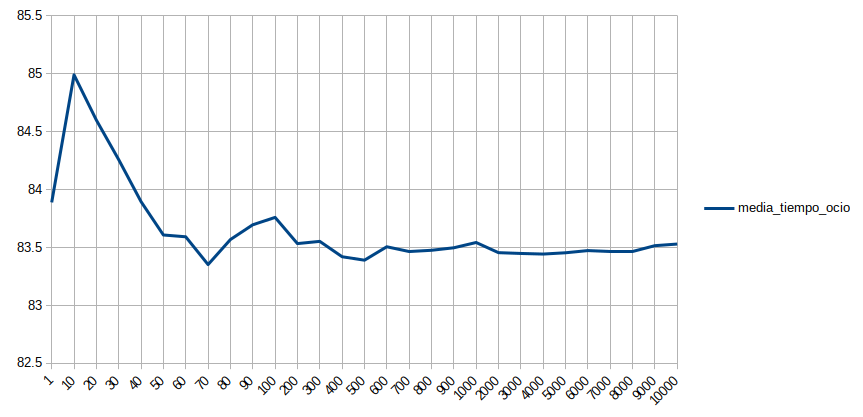
\includegraphics[width=\textwidth]{img/cap-2/valores_estables.png}
  	\caption{Media de tiempo de ocio con respecto al número de simulaciones.}
\end{figure}

Se puede observar que mas o menos a partir de las 700 simulaciones podemos obtener unos resultados relativamente estables.

Tomemos unos valores como referencia de este modelo usando 1000 simulaciones. Los resultados que obtenemos del modelo con un generador de datos exponencial son los siguientes:
\begin{center}
	\begin{tabular}{|c|c|c|}
	\hline
		\textbf{Dato} & \textbf{Media} & \textbf{Desviación típica}\\
	\hline
		Trabajos esperando a ser cargados & 0.018335 & 0.010173\\
	\hline
		Trabajos esperando a ser descargados & 0.015125 & 0.007785\\
	\hline
		Trabajos procesados & 78.153000 & 9.295262\\
	\hline
		Tiempo de estancia de los trabajos & 9.042354 & 0.885916\\
	\hline
		Porcentaje de tiempo de ocio del operario & 83.544128 & 2.355005\\
	\hline
	\end{tabular}
\end{center}


Estos valores los he tomado para poder compararlos ahora con los generadores de datos uniforme y determinísticos.

\section{Diferentes generadores de datos}

He usado las mismas condiciones de ejecución y los datos obtenidos han sido los siguientes:

\begin{center}
	\begin{tabular}{|c|c|c|c|}
	\hline
		 & \textbf{\begin{tabular}[c]{@{}c@{}}Generador\\ determinístico\end{tabular}} & \textbf{\begin{tabular}[c]{@{}c@{}}Generador\\ exponencial\end{tabular}} & \textbf{\begin{tabular}[c]{@{}c@{}}Generador\\ Uniforme\end{tabular}}\\
	\hline
		\textbf{\begin{tabular}[c]{@{}c@{}}Media trabajos\\ esperando carga\end{tabular}} & 0 & 0.018335 & 0.007226\\
	\hline
		\textbf{\begin{tabular}[c]{@{}c@{}}Media trabajos \\esperando descarga\end{tabular}} & 0 & 0.015125 & 0.008656\\
	\hline
		\textbf{\begin{tabular}[c]{@{}c@{}}Media de\\ trabajos procesados\end{tabular}} & 78 & 78.153000 & 78.161003\\
	\hline
		\textbf{\begin{tabular}[c]{@{}c@{}}Tiempo medio de \\ estancia de los trabajos\end{tabular}} & 9 & 9.042354 & 9.069117\\
	\hline
		\textbf{\begin{tabular}[c]{@{}c@{}}Porcent. medio tiempo\\de ocio\end{tabular}} & 83.625 & 83.544128 & 83.515213\\
	\hline
	\end{tabular}
\end{center}

Nos tenemos que fijar en el generador determinístico, que es el que nos va a dar una idea de cómo de cerca se quedan los otros dos de los valores ideales ya que es el que nos proporciona los valores más optimistas del modelo, es decir, nos devuelve el mejor caso posible. Por tanto, se puede apreciar como para el número de simulaciones que realizamos del modelo, los generadores exponencial y uniforme son muy parejos en resultados, y no hay una diferencia demasiado notable entre el uso de ambos.

\newpage
\section{Calidad frente a cantidad}

Se pide que se investigue qué ocurre si cambiamos el procesamiento con un número $x$ de máquinas a una sola máquina que sea $x$ veces más rápida, con un tiempo de proceso de $\frac{\texttt{tproceso}}{\texttt{x}}$. Por tanto, he cambiado el número de máquinas del modelo a sólo una máquina y el tiempo de procesamiento al comentado y los resultados han sido los siguientes (con el mismo número de simulaciones que el comentado al principio del capítulo):


\begin{center}
	\begin{tabular}{|c|c|c|}
	\hline
		 & \textbf{\begin{tabular}[c]{@{}c@{}}Cantidad\end{tabular}} & \textbf{\begin{tabular}[c]{@{}c@{}}Calidad\end{tabular}}\\
	\hline
		\textbf{\begin{tabular}[c]{@{}c@{}}Media trabajos\\ esperando carga\end{tabular}} & 0.018335 & 0.085655 \\
	\hline
		\textbf{\begin{tabular}[c]{@{}c@{}}Media trabajos \\esperando descarga\end{tabular}} & 0.015125 & 0 \\
	\hline
		\textbf{\begin{tabular}[c]{@{}c@{}}Media de\\ trabajos procesados\end{tabular}} & 78.153000 & 79.649002 \\
	\hline
		\textbf{\begin{tabular}[c]{@{}c@{}}Tiempo medio de \\ estancia de los trabajos\end{tabular}} & 9.042354 & 2.302231\\
	\hline
		\textbf{\begin{tabular}[c]{@{}c@{}}Porcent. medio tiempo\\de ocio\end{tabular}} & 83.544128 & 83.421150\\
	\hline
	\end{tabular}
\end{center}

El comportamiento en este caso es muy similar, siendo la espera de la carga un poco mayor que antes, pero el de descarga es 0 debido a la alta velocidad que tiene. En el caso de los trabajos procesados, se procesa de media 1 trabajo y medio más que en el sistema con 10 máquinas. En el caso del tiempo que tardan los trabajos en ser procesados, vemos como la velocidad de media es mucho mayor (como es de esperar). Y por último, el tiempo de ocio no ha variado notablemente.

\newpage
\section{Múltiples operarios}

Ahora, tal y como se pide en el guión, procedo a realizar la implementación de múltiples operarios en el modelo proporcionado para la práctica.

En primer lugar, en el fichero $.h$ lo que haremos será cambiar la variable booleana \texttt{operario\_libre} a una variable entera que será un contador que indicará la cantidad de operarios libres en ese momento. También habrá que crear una variable \texttt{num\_operarios} para indicar el número máximo de operarios que hay disponibles en el sistema.
 
Tras esto, en el fichero $.cpp$ tendremos que actualizar el proceso de inicialización de variables, el cual tendrá que ajustar la variable \texttt{operarios\_libres} (la variable que anteriormente era un bool) al número total de operarios disponibles ya que al inicio se encuentrarán todos disponibles. Una vez hecho esto, tenemos que cambiar todas las veces que aparecía la variable booleana como condición de una sentencia $if$. Lo que habría que hacer es añadirle que la variable sea mayor que 0, o lo que es lo mismo, que haya operarios disponibles que puedan atender las peticiones. Además, hay que cambiar todas las veces que aparezca la asignación $\texttt{operario\_libre} = \texttt{true}$ por un incremento y cuando se le asigne \texttt{false} un decremento. Esto indicará que un operario ha sido ocupado o ha sido liberado.

Con esos cambios ya lo tendríamos todo listo, ahora solo queda probar el sistema con distinto número de elementos. Las distintas combinaciones que voy a probar son las siguientes para realizar la tarea pedida en el guión de prácticas:

\begin{itemize}
	\item{10 operarios con $\texttt{tcarga} = 10$ y $\texttt{tdescarga} = 8$}
	\item{1 operario con $\texttt{tcarga} = 1$ y $\texttt{tdescarga} = 0.8$}
	\item{5 operarios con $\texttt{tcarga} = 5$ y $\texttt{tdescarga} = 4$}
\end{itemize}

\newpage
Los datos obtenidos en las simulaciones (todas con un número de simulaciones de 1000) de todas estas combinaciones son los siguientes:

\begin{center}
	\begin{tabular}{|c|c|c|c|}
	\hline
		 & \textbf{\begin{tabular}[c]{@{}c@{}}10 operarios\end{tabular}} & \textbf{\begin{tabular}[c]{@{}c@{}}1 operario\end{tabular}} & \textbf{\begin{tabular}[c]{@{}c@{}}5 operarios\end{tabular}}\\
	\hline
		\textbf{\begin{tabular}[c]{@{}c@{}}Media trabajos\\ esperando carga\end{tabular}} & 0.000976 & 0.075536 & 0.004666 \\
	\hline
		\textbf{\begin{tabular}[c]{@{}c@{}}Media trabajos \\esperando descarga\end{tabular}} & 0 & 0.048112 & 0.003035\\
	\hline
		\textbf{\begin{tabular}[c]{@{}c@{}}Media de\\ trabajos procesados\end{tabular}} & 77.057999 & 79.570000 & 78.613998\\
	\hline
		\textbf{\begin{tabular}[c]{@{}c@{}}Tiempo medio de \\ estancia de los trabajos\end{tabular}} & 18.495319 & 3.325153 & 9.724446\\
	\hline
		\textbf{\begin{tabular}[c]{@{}c@{}}Porcent. medio \\tiempo de ocio\end{tabular}} & 71.040489 & 70.050056 & 75.504265\\
	\hline
	\end{tabular}
\end{center}

Si interpretamos los datos obtenidos por las tres simulaciones hechas, podemos observar como en este caso la mejor opción es tener 1 operario que sea 10 veces más rapido que cada uno de los operarios del caso de los 10 operarios. Esto lo vemos en la media de trabajos procesados, siento de 79.57 trabajos en el caso de 1 operario frente a las 77.058 en el caso de 10 operarios y 78.61 en el caso de 5 operarios con la mitad de \texttt{tcarga} y \texttt{tdescarga} con respecto del de 10 operarios.

Seguido de esto, tendríamos que también mejoramos el sistema en el caso de usar la mitad de operarios pero el doble de rápidos que en el caso inicial ya que son capaces de conseguir un trabajo más que en la simulación de los 10 operarios. 

\chapter{Análisis de Salidas y Experimentación}

\newpage

\section{¿Cuánto hay que simular?}

Para este primer apartado, el guión pide que comparemos dos configuraciones para el sistema que nos encontramos estudiando:

\begin{itemize}
	\item{La configuracion A con 10 máquinas y 2 operarios y con tiempos de carga y descarga de 3 y 2 minutos.}
	\item{La configuración B con 10 máquinas y 1 operario y con tiempos de carga y descarga de 1.5 y 1 minutos.}
\end{itemize}

En primer lugar se nos pide que probemos el sistema con 1 simulación y repitamos 100 veces para obtener el porcentaje de veces que es preferible un sistema frente a otro. Los datos que obtenemos de hacer esto lo vemos en la siguiente gráfica:

\begin{figure}[H]
\centering
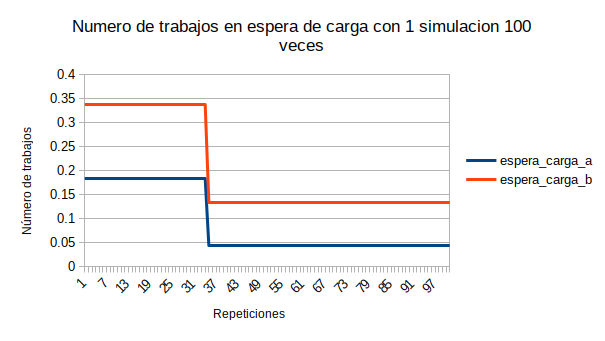
\includegraphics[width=\textwidth]{img/cap-3/espera_carga_1-5-1.png}
\caption{Numero de trabajos en espera de carga con 1 simulación repetido 100 veces}
\end{figure}

En este caso podemos ver que el 100\% de las veces escogemos el sistema A, ya que es el que obtiene menor número de trabajos en espera de carga.

Para el caso de ejecutar 5 simulaciones para cada sistema obtenemos los siguientes resultados:

\begin{figure}[H]
\centering
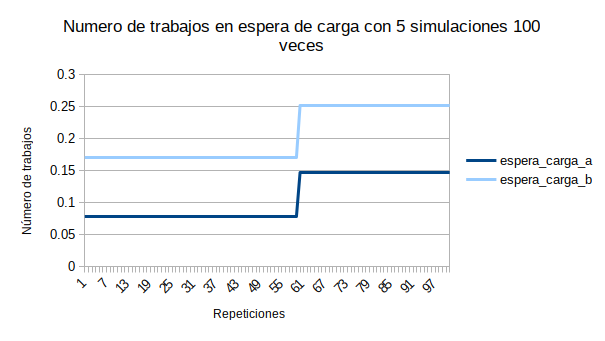
\includegraphics[width=\textwidth]{img/cap-3/espera_carga_1-5-5.png}
\caption{Número de trabajos en espera de carga con 5 simulaciones repetido 100 veces}
\label{}
\end{figure}

Y en este caso también vemos que el 100\% de las veces escogeríamos el sistema con la configuración de A. En el guión se pide que se repita esto mismo pero usando 10, 100, 500, 1000 y 10000 simulaciones. Los resultados los podemos ver en la siguiente gráfica:

\begin{figure}[H]
\centering
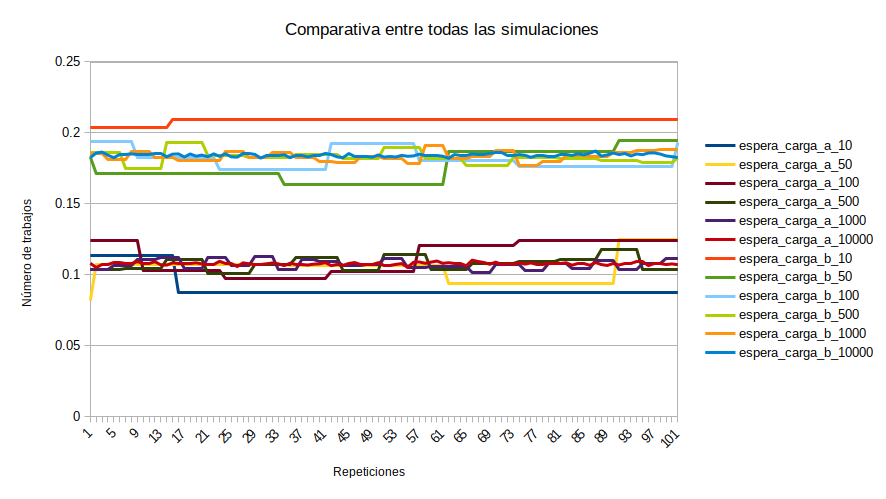
\includegraphics[width=\textwidth]{img/cap-3/espera_carga_todos.png}
\caption{Comparativa entre ambos sistemas con 10, 100, 500, 1000 y 10000 simulaciones.}
\label{}
\end{figure}

La interpretación que sacamos a partir de esta gráfica es que a medida que aumentamos el número de simulaciones, obtenemos unos valores cada vez más precisos. En este caso podemos ver como es la configuración del sistema A el que obtiene un menor número de trabajos en espera de carga para todas las simulaciones, lo que se puede observar si nos fijamos en el conjunto de gráficas de la parte inferior las cuales son todas del sistema A para los distintos números de simulaciones.

\newpage
Por último, el guión pide que se haga lo mismo pero en este caso que comparemos en función del número total de trabajos procesados. En este caso nos tenemos que fijar quién tiene un mayor número de trabajos procesados para saber cuál es el mejor sistema. A continuación se muestran los datos obtenidos en forma de gráfica:

\begin{figure}[H]
\centering
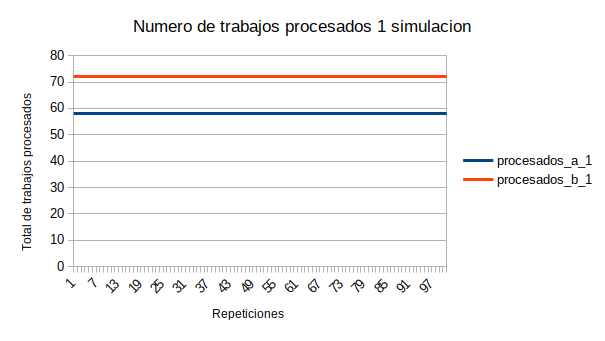
\includegraphics[width=\textwidth]{img/cap-3/ttp_1-5-1.png}
\caption{Total de trabajos procesados con 1 simulación repetido 100 veces}
\label{}
\end{figure}

En esta gráfica podemos ver como es el sistema con la configuración B el que obtiene un mejor resultado el 100\% de las veces que se ejecuta. Vamos a ver ahora qué ocurre si usamos 5 simulaciones 100 veces:

\begin{figure}[H]
\centering
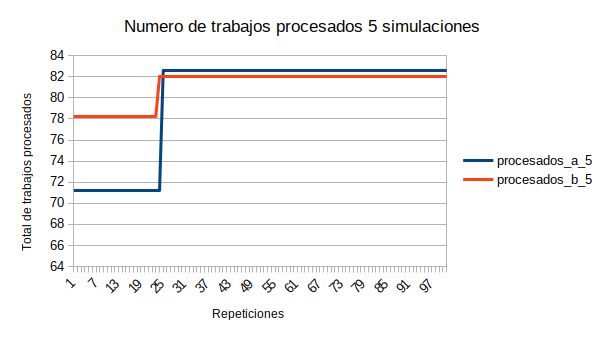
\includegraphics[width=\textwidth]{img/cap-3/ttp_1-5-5.png}
\caption{Total de trabajos procesados con 5 simulaciones repetido 100 veces}
\label{}
\end{figure}

En este caso obtenemos un resultado distinto. En aproximadamente un 27.5\% de las veces obtenemos que el B es el sistema preferible ya que procesa más trabajos que el sistema con la configuración A. En el resto de casos, preferimos escoger el sistema A frente al B.

Ahora en el caso de ejecución de diferente número de simulaciones, si agrupamos todas las representaciones gráficas en una, no podremos ver con claridad qué sistema es mejor que el otro. Voy a poner aquí 3 gráficas que representan exactamente qué es lo que va ocurriendo a medida que aumentamos el número de simulaciones a la hora de elegir un sistema frente a otro.

En la primera figura se representa cómo varían los datos cuando tenemos un número de simulaciones bastante reducido para el sistmea, en el que no sabríamos qué sistema elegir con certeza:

\begin{figure}[H]
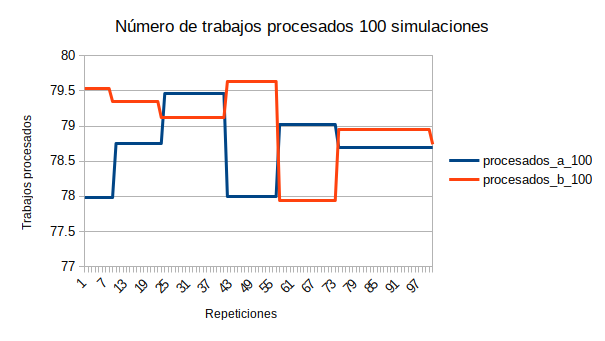
\includegraphics[width=\textwidth]{img/cap-3/ttp_100.png}
\caption{Total de trabajos procesados con 100 simulaciones repetido 100 veces}
\label{}
\end{figure}

En el segundo caso, vemos como con 1000 simulaciones en cada sistema podemos empezar a ver un claro sistema mejor que el otro, que en este caso se va decantando por el sistema B ya que es el que mayor porcentaje de trabajos procesados saca:

\begin{figure}[H]
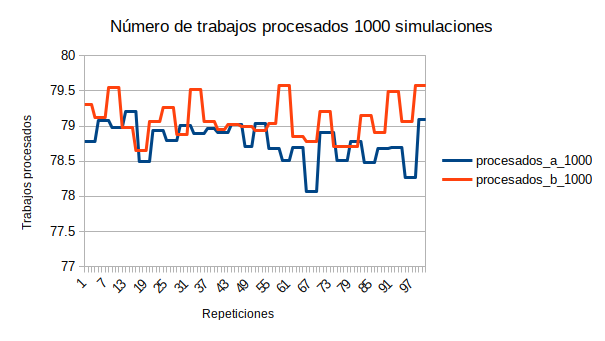
\includegraphics[width=\textwidth]{img/cap-3/ttp_1000.png}
\caption{}
\label{}
\end{figure}

Y por último, en el caso de las 10000 simulaciones para ambos sistemas, aclaramos lo que decíamos con la gráfica de 1000 simulaciones, en la que empezabamos a ver más o menos cómo B iba obteniendo mejores resultados que A pero en algunos casos era A el que lo superaba. Aquí estamos seguros al 100\% de que el sistema que tendríamos que escoger en función del número de trabajos procesados es el sistema con la configuración B.

\begin{figure}[H]
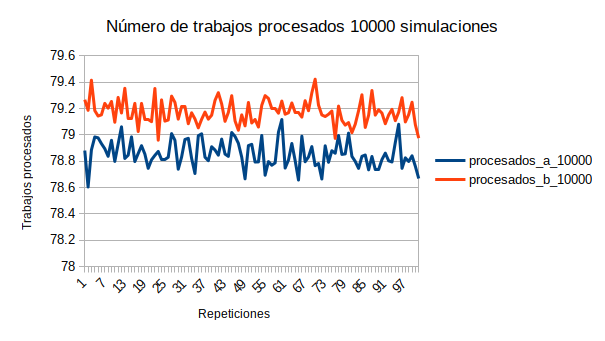
\includegraphics[width=\textwidth]{img/cap-3/ttp_10000.png}
\caption{}
\label{}
\end{figure}
\newpage
\section{Intervalos de confianza}

Para este apartado, el guión de prácticas pide que se haga un estudio sobre si es mejor un sistema con 10 máquinas y 2 operarios con tiempos de carga y descarga de 3 y 2 minutos, respectivamente, o un sistema de 10 máquinas y 1 operario con tiempos de carga reducidos a la mitad con el método de intervalos de confianza tomando como medida el número de trabajos en espera de carga en un caso y el tiempo medio de estancia de los trabajos en otro.

Para ello, lo primero que tenemos que hacer es conseguir las salidas de ambos sistemas para ambas medidas. He usado las medidas proporcionadas de cada sistema con un número de simulaciones de 1000 repetido 100 veces debido a que como se ha visto en el apartado anterior es cuando se obtienen unos valores más estables y reales de cómo funciona una configuración concreta y por lo menos seremos capaces de determinar de mejor manera qué sistema funciona mejor. Con el método de intervalos de confianza, podremos asegurar la elección que hicimos en el apartado anterior.

El $\alpha$ elegido para este caso será un 0.05, con el cual obtendremos un intervalo de confianza al 95\%. Para poder realizar el cáclulo, lo que tenemos que hacer es conseguir la resta de los datos obtenidos por ambas configuraciones, calcularle la media y varianza de todos esos valores y calcular el intervalo con su valor de T de Student con $\alpha = 0.05$ y con $n-1$ grados de libertad. En este caso, tal y como he dicho en el párrafo anterior, usaré un $n=100$ y por lo tanto el calculo de la T-Student se hará con 99 grados de libertad. Los datos finales que he obtenido han sido los siguientes para ambas medidas solicitadas:

\begin{center}
\begin{tabular}{|c|c|c|}
\hline
	\textbf{Medida} & \textbf{Media de (A-B)} & \textbf{Intervalo de confianza}\\
\hline
	\begin{tabular}[c]{@{}c@{}}Número de trabajos\\ en espera de carga\end{tabular} & -0.07660488 & [-0.07685767, -0.07635208]\\
\hline
	\begin{tabular}[c]{@{}c@{}}Tiempo medio de \\estancia en los trabajos\end{tabular} & 1.78550845 & [1.78324745, 1.78776944]\\
\hline
\end{tabular}
\end{center}

Las conclusiones que podemos sacar de estos resultados son que para ambas medidas, al no encontrarse el 0 dentro del intervalo, podemos confirmar que A y B no son iguales con un 95\% de confianza. Como no son iguales, quiere decir que uno es mejor que otro:

\begin{itemize}
	\item{Para el número de trabajos en espera de carga, al tener una media negativa, quiere decir que el mejor sistema es el A ya que obtiene un menor número de trabajos esperando (si la media es negativa significa que B obtiene mayores valores que A)}
	\item{Para el tiempo medio de estancia en los trabajos, tenemos que el sistema B es más eficiente que el A, ya que la media es positiva lo que quiere decir que B termina antes los trabajos que A.}
\end{itemize}


\section{Comparación de más de dos sistemas}

En el guión de prácticas también se pide que se comparen cuatro configuraciones distintas para ver qué sistema es el mejor. La medida de rendimiento a utilizar es el tiempo medio de estancia de los trabajos.

Para realizar esta comparación, usaré el método que aparece en las diapositivas de teoría, el método de selección del mejor entre $k$ sistemas. Para poder aplicar dicho método de comparación hay que escoger una serie de parámetros:

\begin{itemize}
	\item{Lo primero que tenemos que elegir es un valor de $P^*$, cuya elección depende la precisión que queramos del resultado. Obviamente queremos una buena precisión para elegir el mejor sistema, por lo que usaremos una probabilidad suficientemente alta. En este caso usaré un valor de probabilidad del 95\% y por tanto un valor de $P^*=0.95$.}
	\item{Tenemos que elegir también el valor de la indiferencia. En este caso elegiré $d^*=1$.}
	\item{El valor de $n_0$ que escogeré será de 40}
	\item{Por lo tanto, el valor de $h_1$ que tendré que escoger es 3.003 (ya ue va en función del valor de $k$ y $P^*$.}
\end{itemize}

Los resultados de $X^p_i(N_i)$ que he obtenido para cada sistema son los siguientes: 

\begin{center}
\begin{tabular}{|c|c|}
\hline
	\textbf{Sistema} & \textbf{$X^p_i(N_i)$}\\
\hline
	\textbf{10 máquinas 1 operario} & 1.454\\
\hline
	\textbf{10 máquinas 2 operario} & 3.035\\
\hline
	\textbf{10 máquinas 5 operario} & 5.551\\
\hline
	\textbf{10 máquinas 10 operario} & 10.419\\
\hline
\end{tabular}
\end{center}

Para poder analizar esos resultados, tenemos que ver qué configuración es la que tiene un valor menor de $X^p_i(N_i)$ ya que nos interesa el sistema que tenga menor tiempo medio de estancia de los trabajos, lo que indicará que procesa el trabajo con mayor velocidad que el resto.

Por lo tanto, teniendo en cuenta ésto, la mejor configuración es la de 1 operario con tiempos de carga y descarga de 0.6 minutos y 0.4 minutos respectivamente.

\end{document}

